Выберем 3 модели - линейная, логистическая и ridge регрессии, обучим на них классификатор и сравним качество
\begin{table}[h]
\centering
\begin{tabular}{lcccc}
\toprule
\textbf{Размер выборки} & \textbf{Модель} & \textbf{Precision} & \textbf{Accuracy} & \textbf{Recall} \\
\midrule
\multirow{3}{*}{N=25} 
 & Logistic & 0.730 & 0.749 & 0.789 \\
 & Linear & 0.734 & 0.752 & 0.789 \\
 & Ridge & 0.734 & 0.752 & 0.789 \\
\midrule
\multirow{3}{*}{N=100}
 & Logistic & 0.916 & 0.919 & 0.923 \\
 & Linear & 0.906 & 0.919 & 0.935 \\
 & Ridge & 0.906 & 0.919 & 0.935 \\
\midrule
\multirow{3}{*}{N=500}
 & Logistic & 1.000 & 1.000 & 1.000 \\
 & Linear & 1.000 & 1.000 & 1.000 \\
 & Ridge & 1.000 & 1.000 & 1.000 \\
\bottomrule
\end{tabular}
\end{table}

\noindent В качестве самой удобной и не проигрывающей по качеству модели выберем логистическую регрессию и дальше будем анализировать дисперсию и важность характеристик относительно нее.\\


\textbf{Проведем кроссвалидацию для оценки дисперсии метрик}\\

\hspace*{-1cm}
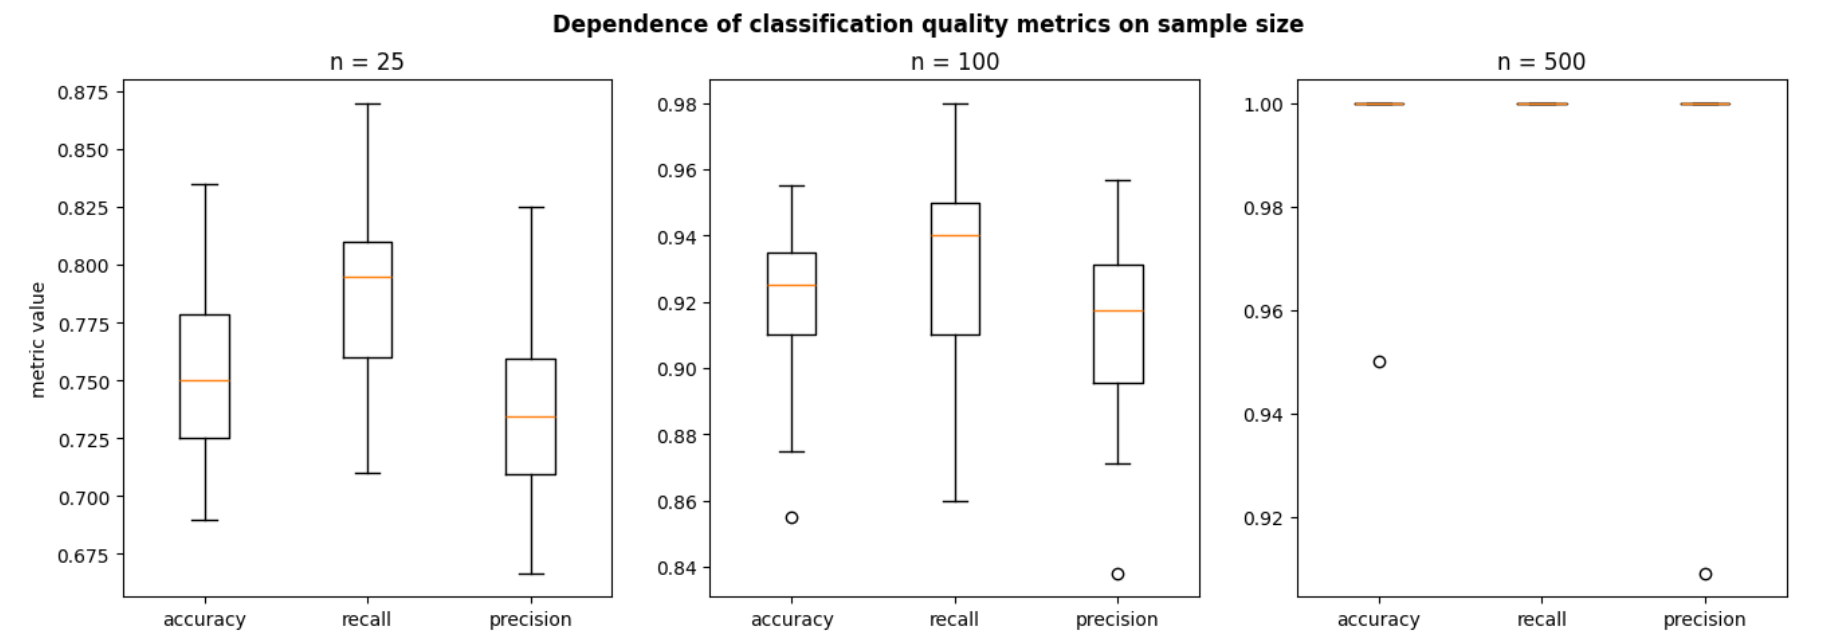
\includegraphics[width=1\textwidth]{Part-II-Ivanova/dispers.png}\\ 


\begin{table}[h]
    \centering
    \begin{tabular}{lcccc}
    \toprule
    \textbf{Размер выборки} & \textbf{Метрика} & \textbf{Среднее} & \textbf{Дисперсия} \\
    \midrule
    \multirow{3}{*}{N=25} 
     & Accuracy & 0.75 & 0.001028 \\
     & Recall   & 0.79 & 0.001366 \\
     & Precision & 0.73 & 0.001303 \\
    \midrule
    \multirow{3}{*}{N=100}
     & Accuracy & 0.92 & 0.000411 \\
     & Recall   & 0.94 & 0.000906 \\
     & Precision & 0.91 & 0.000593 \\
    \midrule
    \multirow{3}{*}{N=500}
     & Accuracy & 0.99 & $4 \times 10^{-5}$ \\
     & Recall   & 1.00 & 0.0 \\
     & Precision & 1.00 & 0.00016 \\
    \bottomrule
    \end{tabular}
\end{table}
\newpage
\noindent \textbf{Вывод :}\\
При увеличении размера выборки, дисперсия снижается достаточно быстро.\\
\\
\textbf{Оптимальный размер:} \\
В зависимости от задачи можно использовать:
\begin{itemize}
    \item граф на 100 вершинах (если нужны быстрые вычисления и неплохое качество) 

    \item граф на 500 вершинх, если нужна высокая точность, и есть время на вычисления (т.к. вычисления на графе для 500 вершинах кратно увеличиваются)

\end{itemize}

\restoregeometry